%! TEX root = ./main.tex

\lecture{25}{Week: 13}{Direct Memory Access}

For large data transfers we should not use programmed I/O but direct memory access. This way the data transfer is not routed via the CPU but over a dedicated DMA controller. This way the CPU can do different things in the meantime. The CPU is still responsible for initiating the transfern but once this is done the DMA controller takes over. When done, the DMA controller interrupts the CPU.

This is build into the south bridge of processors.

\paragraph{DMA Transfer}
The DMA controller sits on the PCI bus, to which the disk controller is connected. This represents the schematics of a rather old PC.

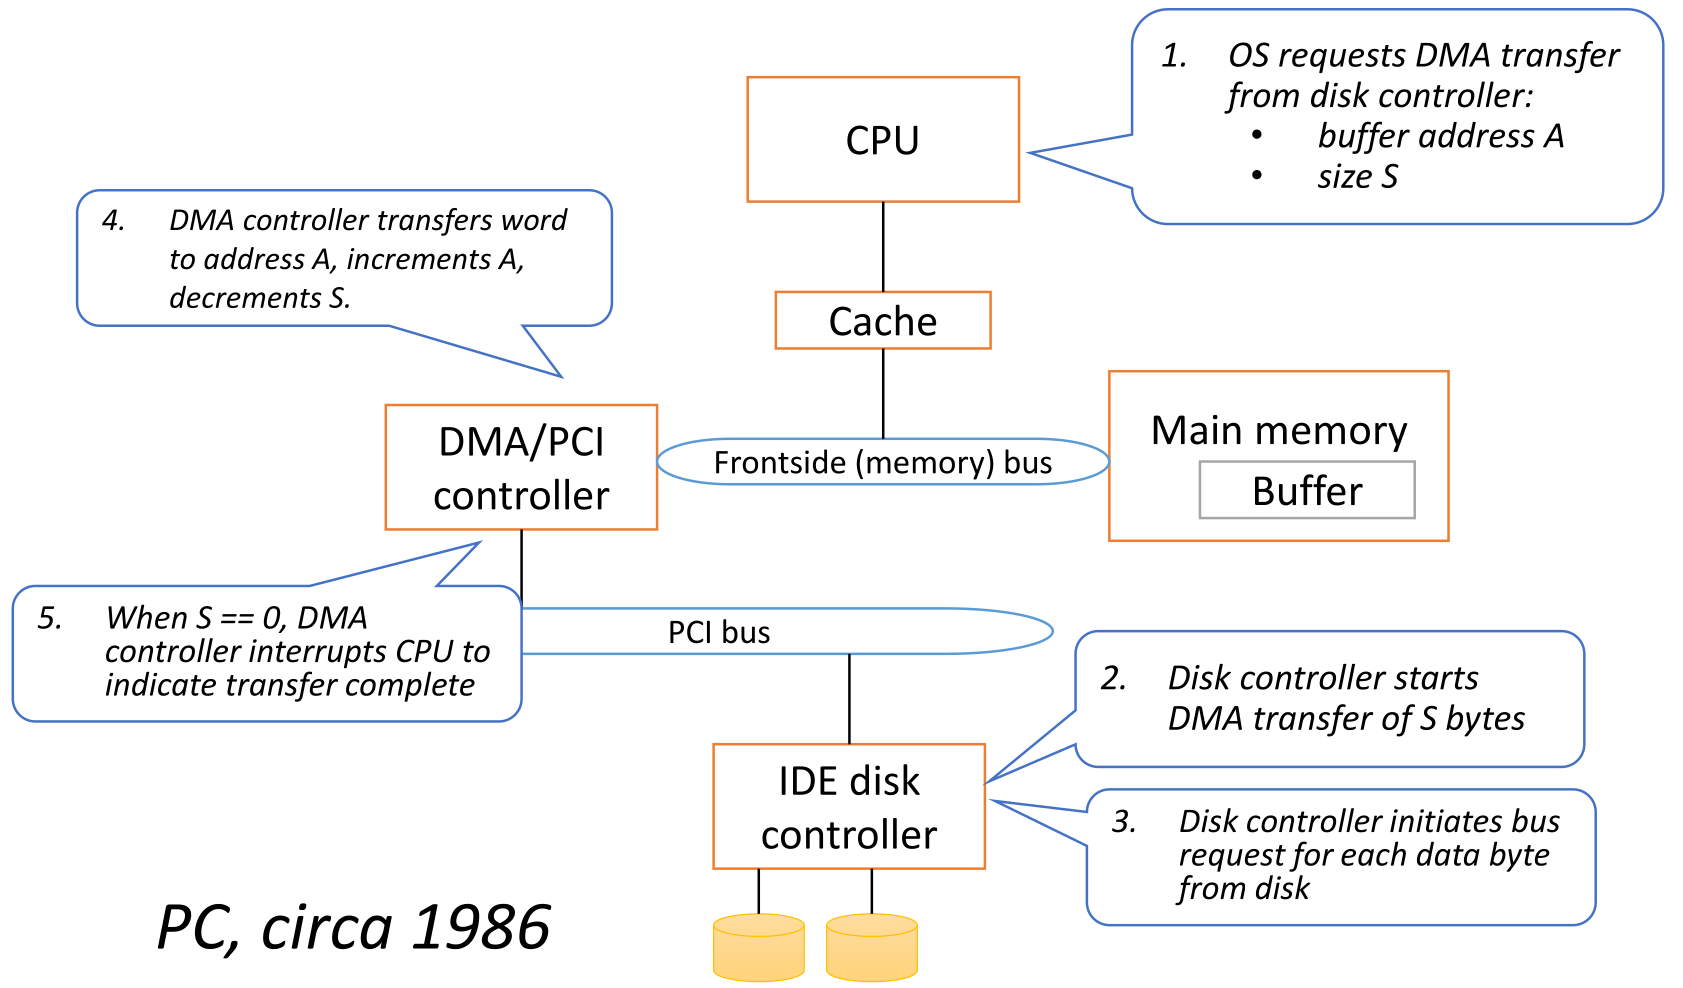
\includegraphics[width=0.8\textwidth]{25_DmaTransfer.png}

In the following the steps for a CPU initiated DMA transfer are depicted. The OS is trying create a file which gets memory mapped from the disk to main memory.

\begin{enumerate}
    \item The file should get the content of a particular buffer address A of size S. We signal the disk controller that we want to read buffer address A of size S.
    \item The disk controller starts to transfer S bytes. Instead of communicating with the CPU it sends the data to the DMA controller.
    \item For each byte the disk controller wants to send, it does a bus request.
    \item The DNS controller listens on the bus and transfers the data words it receives to address A (in the main memory). The it increments A and decrements S.
    \item When \code{S == 0} the DMA controller interrupts the CPU to indicate that the transfer is complete.
\end{enumerate}

The DMA controller is not a very complex hardware component and can be seen as a finite state machine.

\paragraph{Advantaged/Disadvantages}
The DNA controller decouples data transfer from processing. So, the CPU does not have to deal with copying data from/to devices. This way the cache is also not polluted. Further, the OS can decide when to schedule disk reads/writes and work in parallel to these disk actions.

Possible disadvantages are that there is a possibility of bus contentions during transfer. For small transfers the setup overhead may dominate. But in general this is not a problem and it is widely used.

\paragraph{DMA and Caches}
DMA may make memory inconsistent when it change memory blocks which are cached by the CPU. Possible solutions to this issue are:

\begin{itemize}
    \item We can mark pages as non-cacheable (similarly as we did with regions of memory which correspond to device drivers). This is not a great idea since once the transfer is complete we want to be able to cache this data.
    \item Since de DMA controller sits on the main memory bus it can snoop and interact with the cache coherency protocol. Obviously, this does only work for SMP systems.
    \item The OS can explicitly flush and invalidate regions of memory. This mean that the OS writes addresses, which are about to get written to disk by the DMA controller back to memory. And it marks regions of memory as invalid when they are going to get overwritten by the DMA.
\end{itemize}

\paragraph{DMA and Virtual Memory}
DMA uses physical addresses while the user and OS deals with virtual addresses. Therefore, the OS and device drivers must manually translate between virtual and physical addresses. This is more complicated than it seems at first glance because contiguous virtual addresses may not be contiguous in physical addresses. Therefore, SMA controllers support scatter and gather. This means that the controller is not given a base address and a size but rather a list of addresses. This way we can still access a large portion without it must be contiguous.

Most modern systems have a IOMMU (IO memory management unit) which is, as the regular MMU, responsible for address translation but for IO devices (DMA writes from devices). This IOMMU is programmed by the OS because it must coincide with the address space and the MMU.

Besides the discussed purpose, IOMMU has many other purposes.

\paragraph{Evolution of IO Devices}
\begin{enumerate}
    \item Drivers relied on programmed IO and polling was used to get device states.
    \item Polling is too slow so interrupts are used to notify the CPU for certain actions.
    \item CPU spends too much time copying, therefore DMA controllers were used to offload this task from CPUs and allow them to happen in parallel.
    \item Too many interrupts slow down the controller and CPU and resynchronisation is required (do not know that this means).
    \item Devices become more complex and are almost a processor themselves (e.g. GPU).
\end{enumerate}


\subsubsection{Device Drivers}
A basic model of how drivers interact with the OS are depicted below.

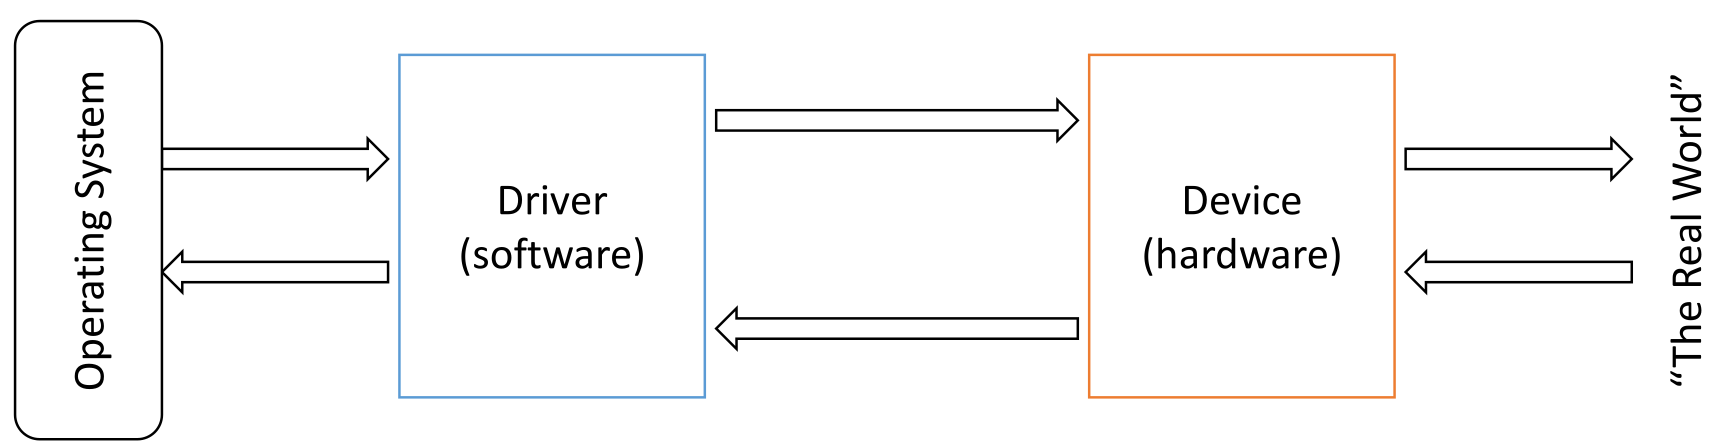
\includegraphics[width=0.8\textwidth]{25_BasicModel.png}

Drivers are often considered to be part of the OS.

The driver as well as the device can be considered as a state machine which take action depending on their state as well as the state of the device. Date must be transfered between the two and events are signal state transitions.

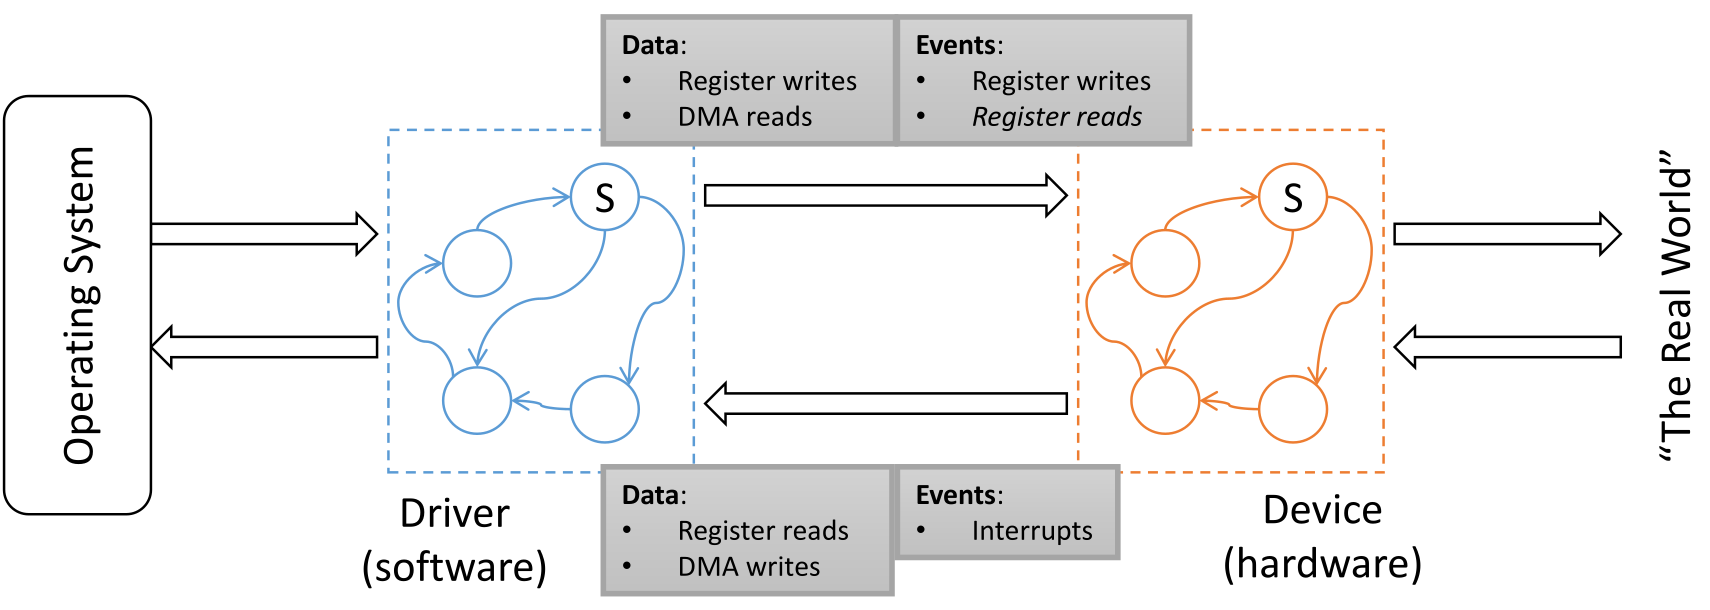
\includegraphics[width=0.8\textwidth]{25_BasicModelStateMachine.png}

\paragraph{Device - CPU Communication}
As discussed, there are multiple ways how a device can communicate with the CPU:

\begin{enumerate}
    \item CPU -> Device; The CPU can write device registers. This communication is synchronous.
    \item CPU <-> Device; The CPU can read device registers. This communication is synchronous.
    \item Device -> CPU; The device requests an interrupts. This communication is synchronous.
    \item Shared memory is used for actually transferring data. It is asynchronous, meaning that not both actors need to be available on the same time.
\end{enumerate}

\subsubsection{Buffer Rings and Descriptor Rings}
Buffer / descriptor rings are visualized as a ring with two pointer to it. The \textit{Head} pointer is the pointer of the device and the \textit{Tail} pointer is controlled by the CPU. Both pointers can move independently as soon as data is added or read.

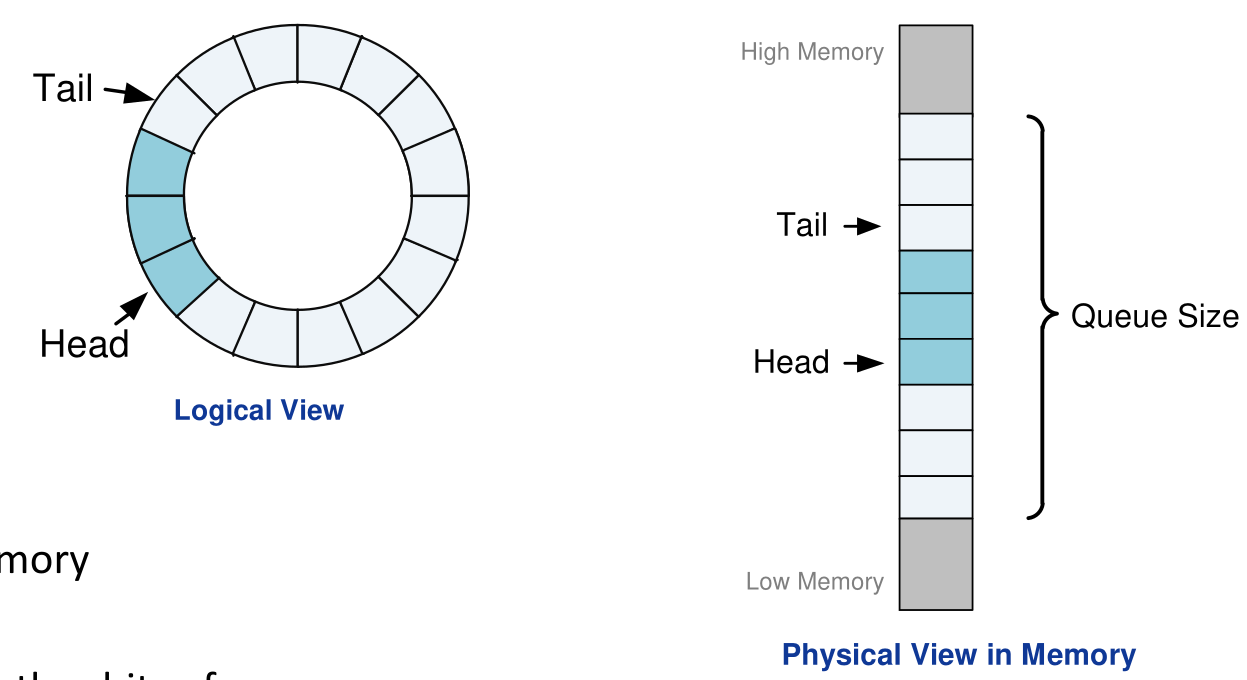
\includegraphics[width=0.8\textwidth]{25_RingBufferOverview.png}

The buffer is of limited size and therefore it is crucial to check if the is space. As a data structure, it is implemented as a queue with two pointers and a fixed size. The entries are contiguous in memory. Often, the values of the queue are pointer to other places in memory to allow to store entries of different size.

Each descriptor is either owned by the CPU or the device. The one who owns a descriptor is the one who can read it.

Once everything is initialized by the CPU, there is no need for further communication and synchronisation between the device and the CPU (expect for underruns and overruns). When writing or reading, the only thing the two agents have to make is that they read/write a entry which belongs to them (i.e. that they are not causing an overrun or underrun).

In essence, these buffers are producer-consumers queues which are not based on mutexeses, locks etc. for synchronisation but relay on messages based on reading/writing registers or interrupting each other.

Often, there are two buffer rings in a system, one for reading/receiving (CPU reads from device) and one for writing/transmitting (CPU writes to device).

\paragraph{Transfer}
The following image shows a buffer ring for transmitting (writing) data.

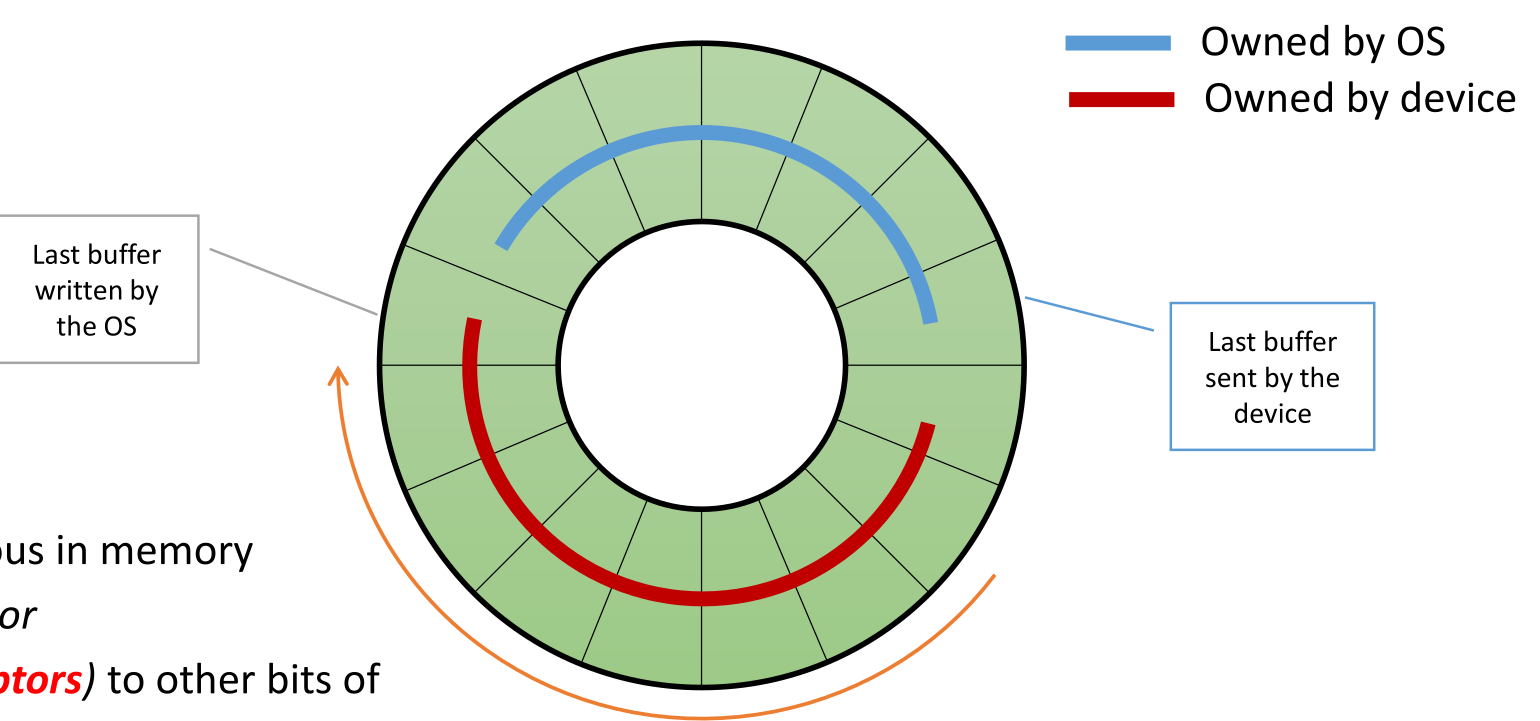
\includegraphics[width=0.8\textwidth]{25_RingBufferZoomIn.png}

\paragraph{Receive}
The following image shows a buffer ring for receiving (reading) data.

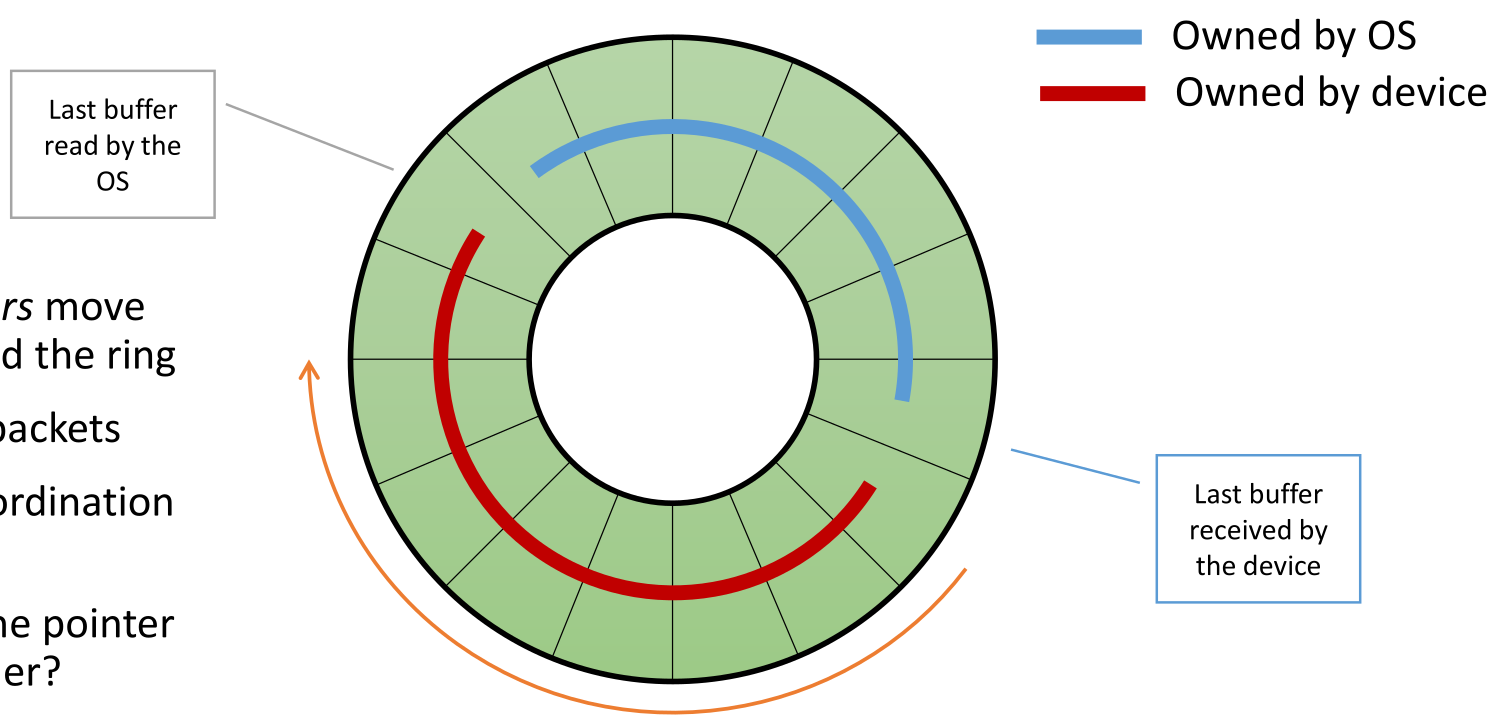
\includegraphics[width=0.8\textwidth]{25_RingBufferReceive.png}

\paragraph{Advantages}
Most modern systems use such buffer descriptors (instead of reading and writing directly to memory). This pointers provide a level of indirection. In addition to the raw data, also some metadata like error messages are transmitted. So we have to ability to write them to a separate buffer. This way data and metadata is not mixed. Further advantages are that we are much more flexible where data is stored since as we said, the entries of the ring can be pointers them selves. Buffers can be of different size and they can even resize dynamically.

\paragraph{Overruns and Underruns while Receiving}
While the CPU is receiving data, if the buffer gets full and the device does not have space for new packages the device starts to discard new packages which are coming in (it does not overwrite old packages). There may be some other buffers which kind of act like a backup buffer once the "main" buffer is full. In general this is not that bad when packages are lost since there are protocol that detect that and can request resending of this package. The CPU must signal the device must wait (tell the device our status).

When the CPU has read all data of the buffer, it must wait. One solution to deal with that is to spin poll, i.e. spin loop and check if there is new data to process. But this keeps to CPU busy and it cannot do anything else in the meantime. Another solution is to signal to the device that is should interrupt the CPU once there is new data is the buffer. This way the CPU can deal with other things in the meantime.

\paragraph{Overruns and Underruns while Transmitting}
When the CPU is writing to the buffer and the buffer is full, it has to wait for the device to make space on the buffer for further writes. Again, it can spin poll or tell the device that it should interrupt it once there is again space in the buffer.

If there are no more packages for the device to receive it must wait. The device could continue to poll the buffer till there is new data to read or it could signal the CPU to wake it up when there is more data in the buffer and go to sleep.

\subsubsection{More Complex Devices}
\paragraph{Network Adapter/Network Interface Card (NIC)}
NICs are often connected to the PCIe bus. It has a integrated DMA engine and has a link interface where it received network packages.

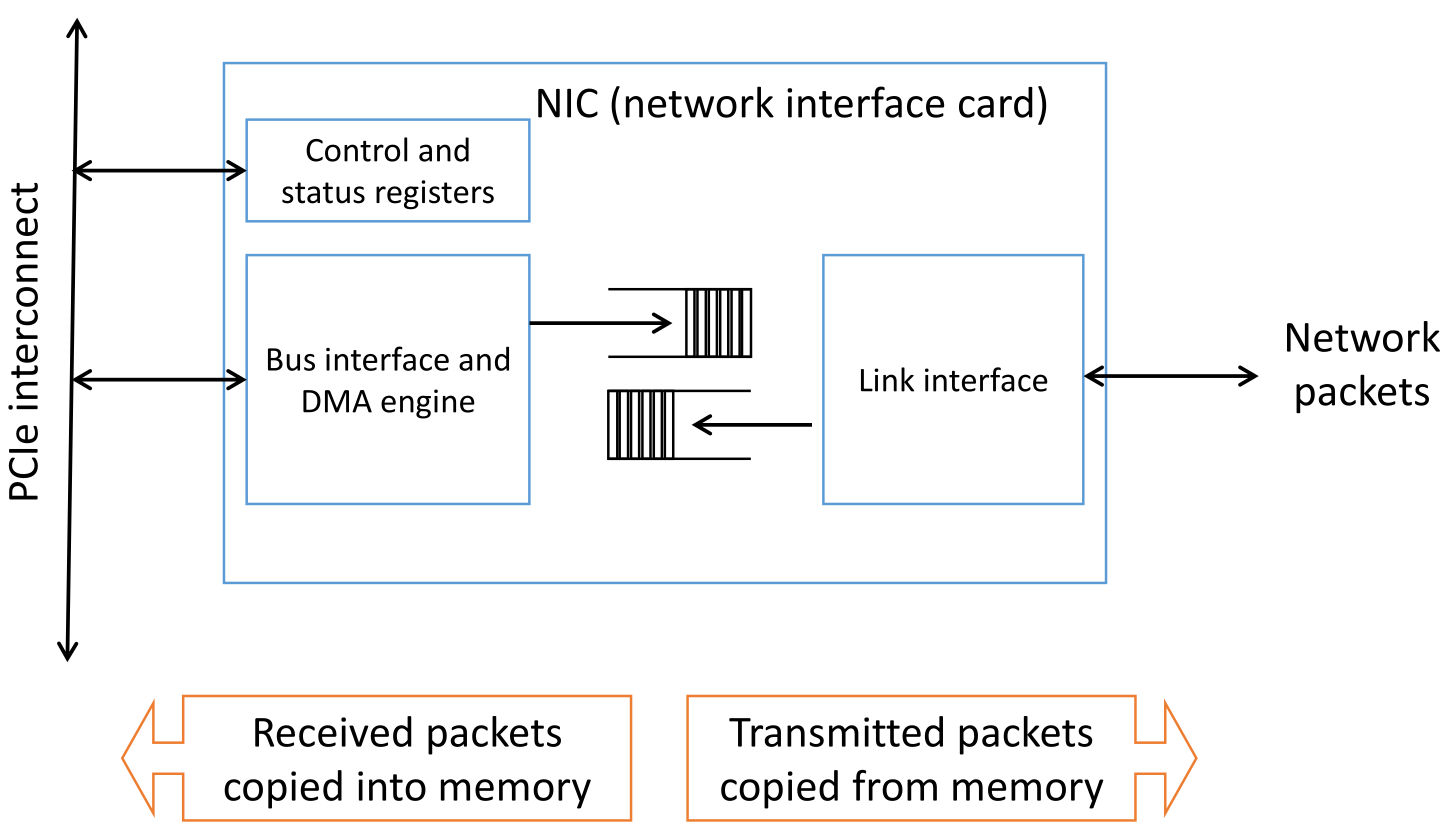
\includegraphics[width=0.8\textwidth]{25_Nics.png}

The NIC transmits data from memory to the network and moves packages received from the network to memory.

\paragraph{Example: DEC "Tulip" Fast Ethernet Adaptor}
This device is very old but  very well documented. It illustrated all basic principles of more complex devices.

As with the UART, we have again different registers to communicate with the device. For example receive/transmit poll demand are flags which indicate that there is data to read/write. The Receive/Transmit list base addresses are the base address of the buffers. The interrupt enable is a flag to enable/disable interrupts.

CSR13 and CSR14 are not listed below. That is because according to the data sheet they are not meant to be accessed by the CPU and changing them can have unexpected results.

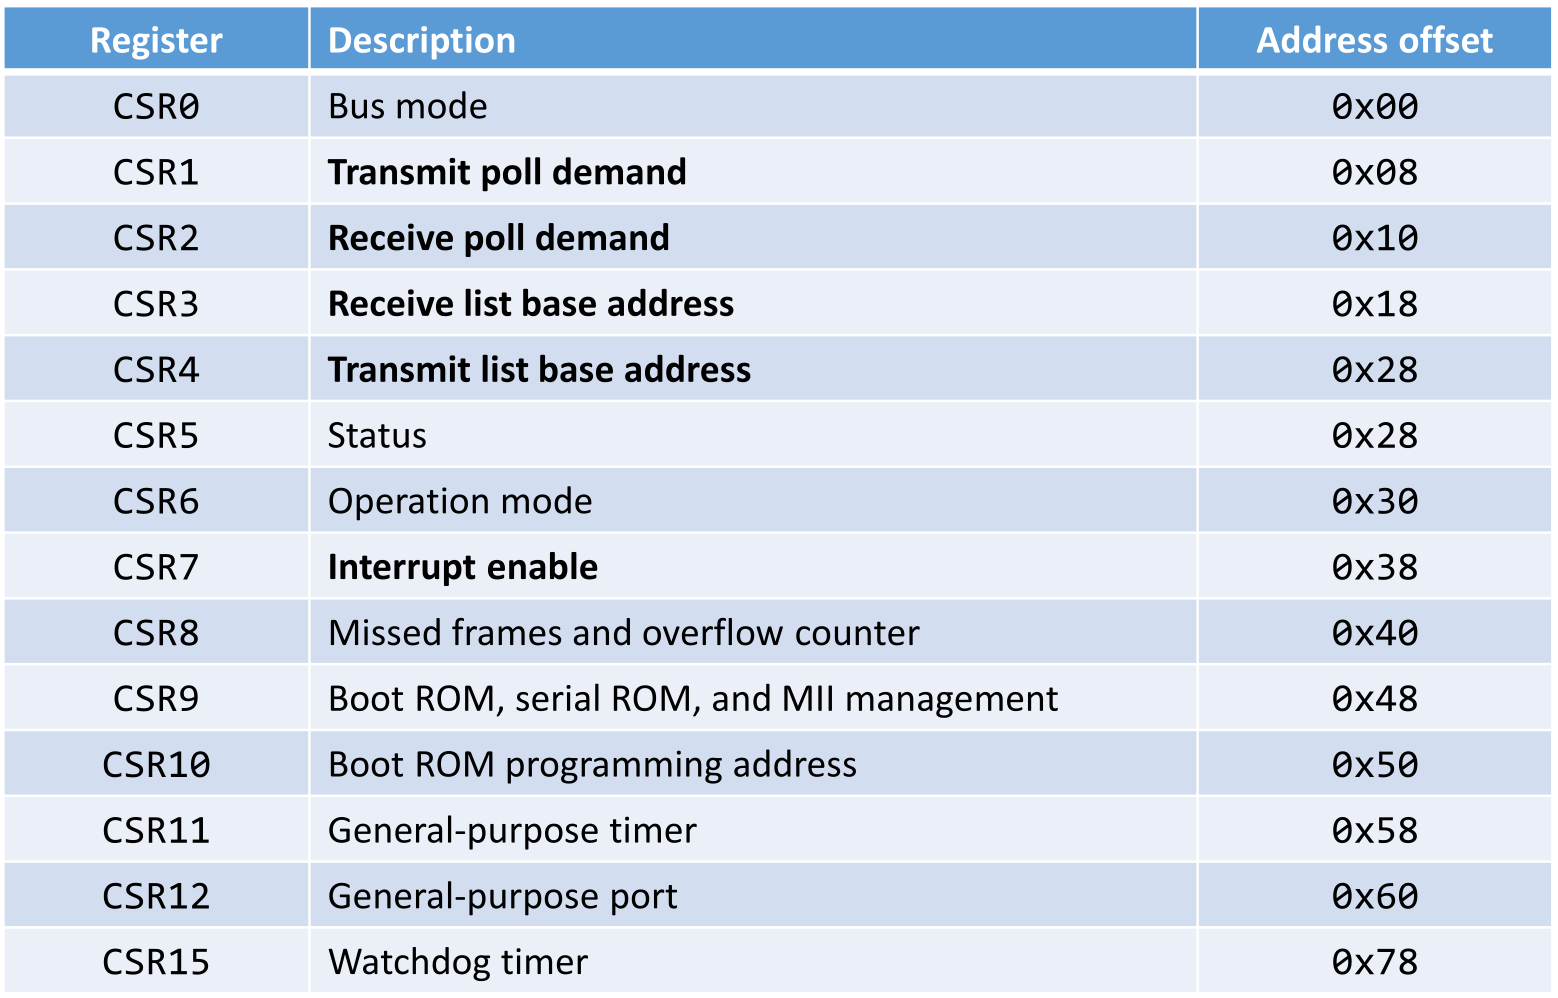
\includegraphics[width=0.8\textwidth]{25_DecRegister.png}

The descriptors of this device look as follows. They have space for two buffer addresses. There are status bits and own bits which indicate if the buffer are device or hardware owned (do not know what this means). The two size count bits tell the size of the two buffers. The control bits are used 

The second address buffer can either act as a buffer or a liked list. But in general the two are used for transmitting and one for receiving. This is controlled by the RSH bit. The FS and LS flags help to figure out the size of the queue.

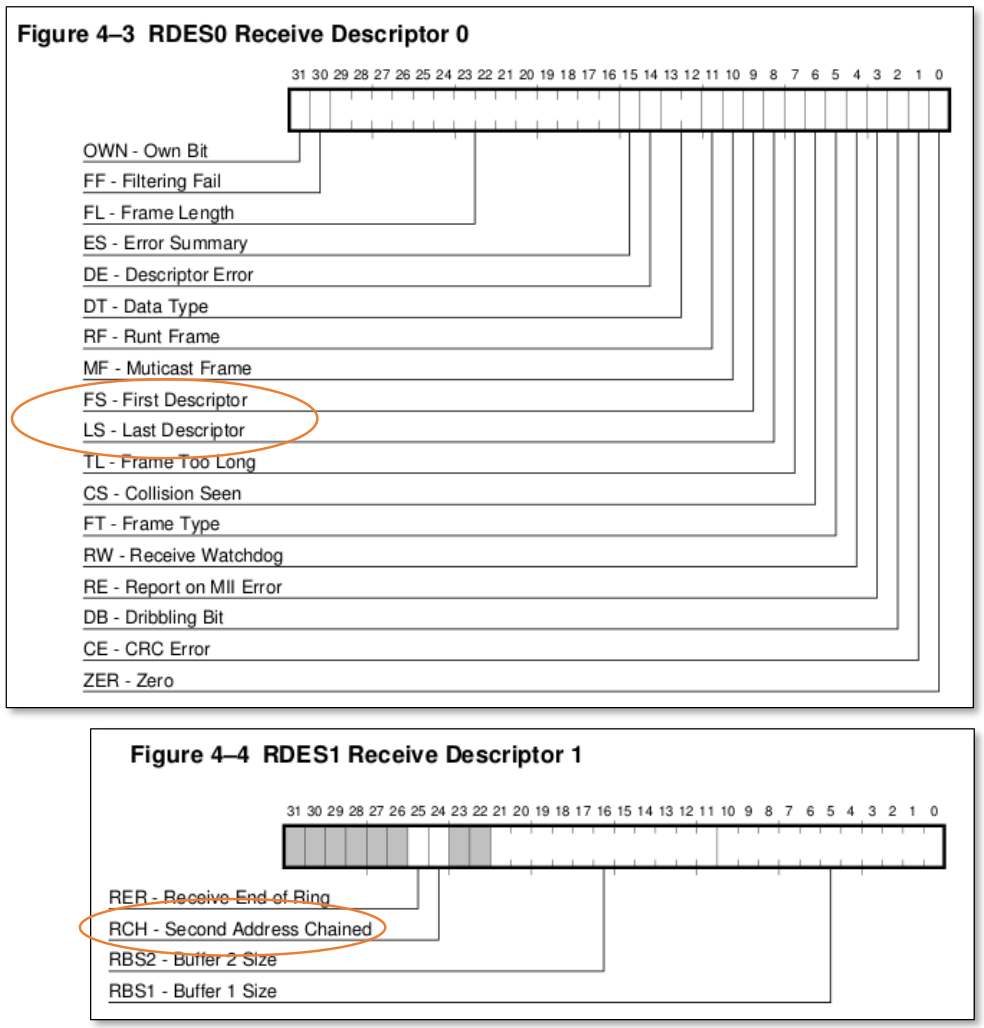
\includegraphics[width=0.8\textwidth]{25_DecControlBits.png}

\paragraph{Descriptor Ring - Normal Mode}
The base address points to the first descriptor. Then we have the whole chain of descriptors, where each holds a pointer to some other region in memory.

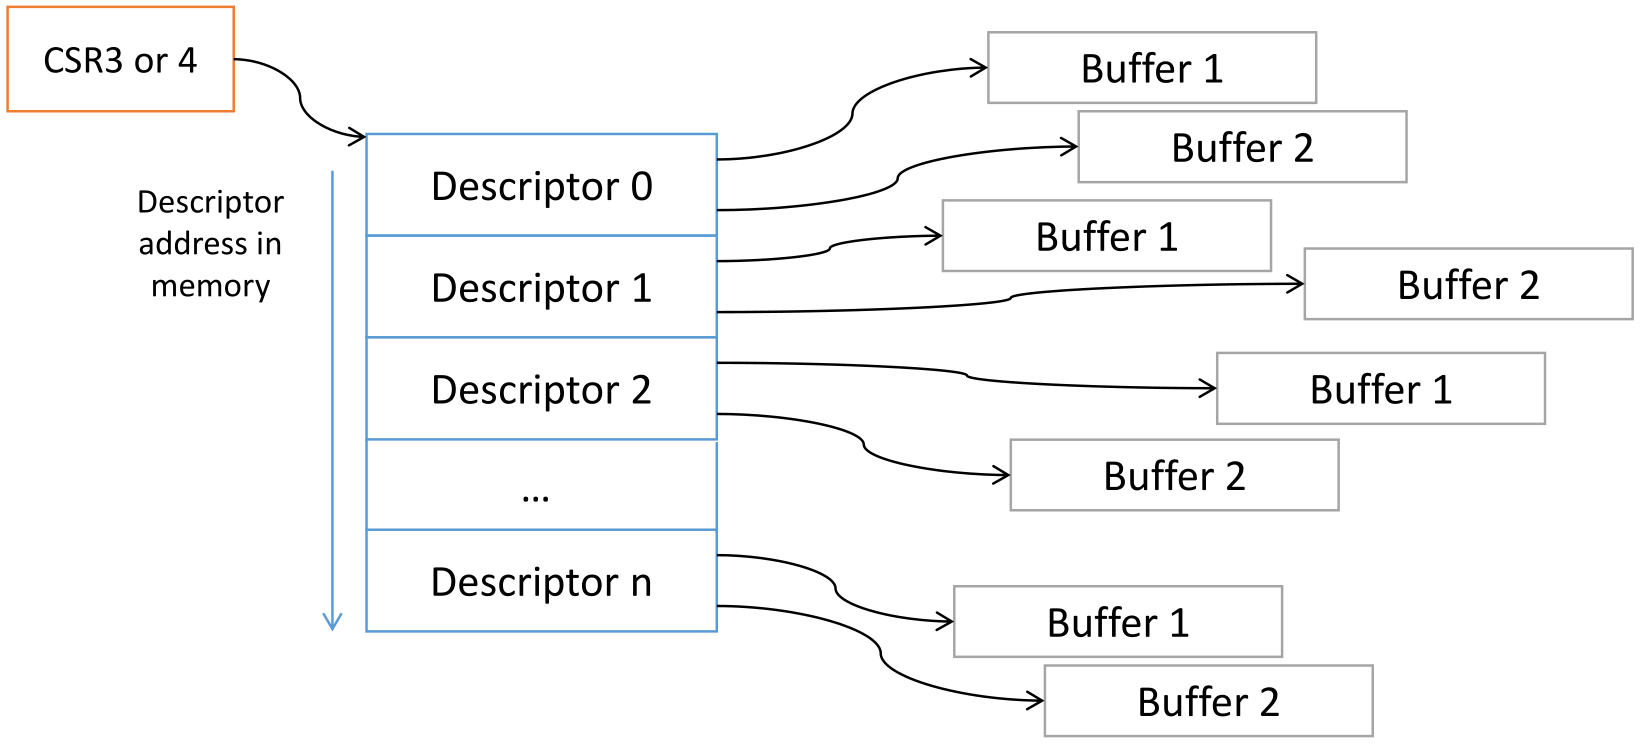
\includegraphics[width=0.8\textwidth]{25_DecRingNormal.png}

\paragraph{Descriptor Ring - Chain Mode}
In this mode the base address points to the first descriptor. This node then hold a pointer to some data as well as a pointer to the next descriptor. In this case the descriptors are not contiguous in memory. 

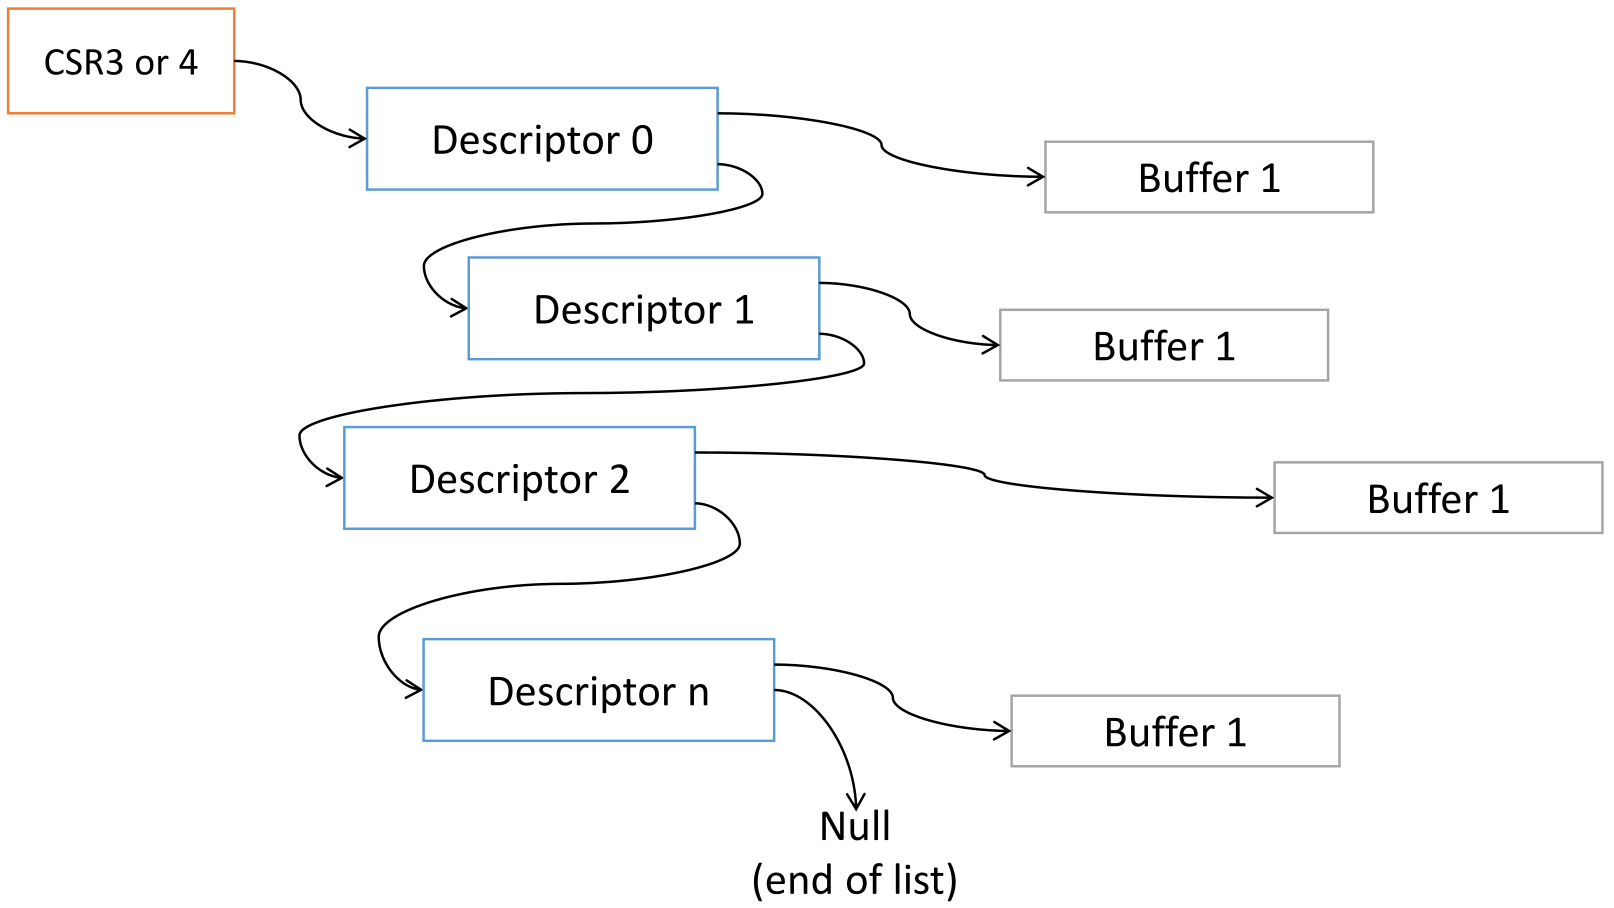
\includegraphics[width=0.8\textwidth]{25_DecDescriptorRingChain.png}

\subsubsection{Device Initialisation}
Before a device can be used, the driver must initialize it. We said that the driver as well as the device are some kind of statemachine. When plugged in, we do not know what state a device is in. So we have to put it into a known state. In general, this requires the following steps:

\begin{enumerate}
    \item Wait for the hardware to settle down.
    \item Stop the device from doing anything (sending interrupts, DMA, sending packages etc.).
    \item Create the shared data structure and tell the device where it is by writing the address into some register. 
    \item Start the device by writing some registers.
\end{enumerate}

\paragraph{IO State Machines; Transfer (hardware side)}
We are looking at the statemachine of the device and assume that we send packages to the device.

The device is either in Stopped or Running state. To start the device, the driver must write a certain register. In response, the device looks at the buffer and DMA reads the next descriptor. If the next descriptor owned bit indicates that the descriptor is owned by the device, it DMA reads the buffer and sends the package. Then the device DMA writes the owned flag to make it belong to the OS again. Afterwards, it calculates the address of the next descroptor (depends if we use a buffer or a linked list). The device repeats this procedure till the next descriptor is owned by the OS. In that event, it goes to the stopped state and notifies the CPU that it waits for an interrupt.

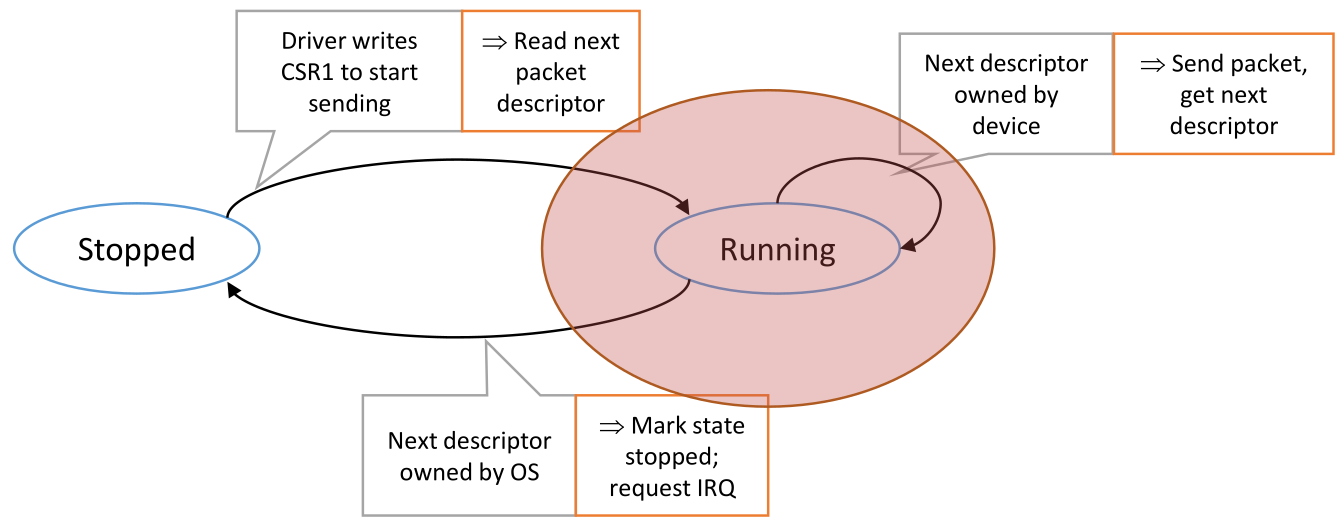
\includegraphics[width=0.8\textwidth]{25_StateMachineDevSend.png}

\paragraph{IO State Machines; Transfer (software side)}
We are looking at the statemachine of the driver and assume that we send packages to the device.

The driver has three different states; stopped, waiting and running. We are in the stopped state and we have a package to send. So we read the descriptor and check the owned bit in order to make sure that there is space for us to write. We copy the data to the buffer and mark it as owned by the device. This brings us to the running state.

Back in the stopped state, if we want to send a package and hence, read the owned bit of the next descriptor in order to make sure it is ours. Now it case that it is not our (i.e. the buffer is full), we get into the waiting state and indicate to the device that we want to get interrupted by setting a register. When the device interrupts us, we copy the data into the descriptor and mark it as owned by the device.

If we are in running state, read a next descriptor and it is owned by us, we copy the data into the descriptor and go to the next descriptor. We stay in the running state as long as we can read next descriptors. From the running state, we go into waiting if we want to send data but the buffer is full, or we go into stopped once we do not want to send any more data.

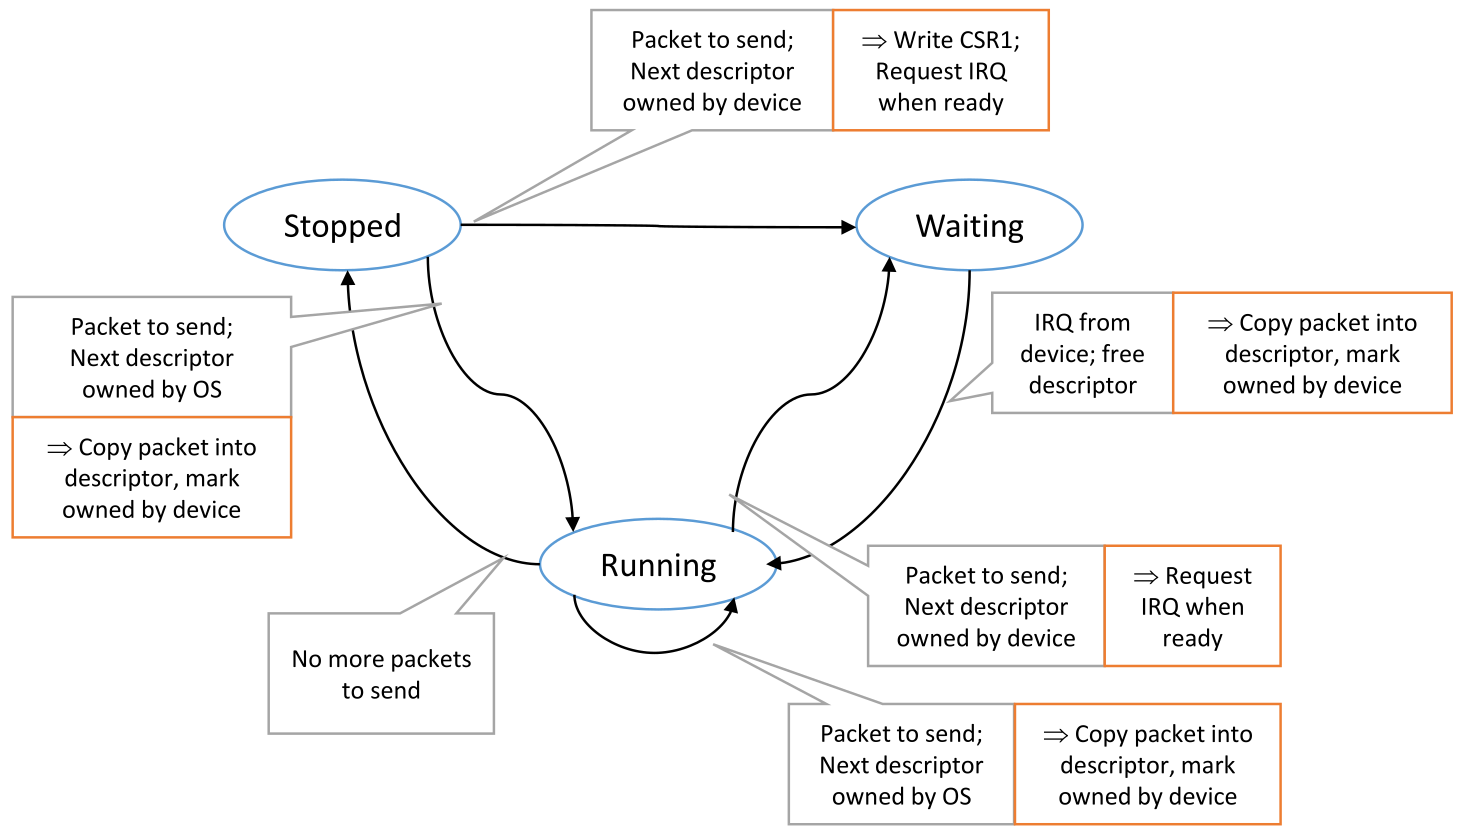
\includegraphics[width=0.8\textwidth]{25_StateMachineOsSend.png}


\paragraph{Avoid Cache Problems}
On x86 hardware, PCI-based DMA listens to the memory bus and ensures this way that the cache are consistent. On all other hardware we have to:

\begin{itemize}
    \item On DMA read a certain address. Before the DMA reads, we have to make sure that the lastest changes of that address are in memory (DMA reads memory). We do this by flushing (write dirty data back to memory) the addresses. After the DMA read, the CPU invalidates (discard all lines from the cache) the cache for the address. This is done to prevent using outdated descriptors (on a DMA read, the device also writes to memory).
    \item On DMA write a certain address. Before the DMA write, we flush or invalidate the whole (I guess) cache to make sure that memory has the latest changes. After the write we invalidate the whole cache in order to fetch the new data from memory.
\end{itemize}

\paragraph{IO State Machines; Receive (software side)}
We have two states, stopped and running. When in stopped, we get an interrupt from the device that new packages have arrived. We acknowledge the interrupt and read the package. We change the owned bit to indicate that is owned by the device. This brings us into the running state. When in this state, we keep reading descriptors, as long as they are owned by us. If the next descriptor is owned by the device, we write to a certain register to indicate that we are stopped are request a interrupt when there is new work. This brings us to the stopped state.

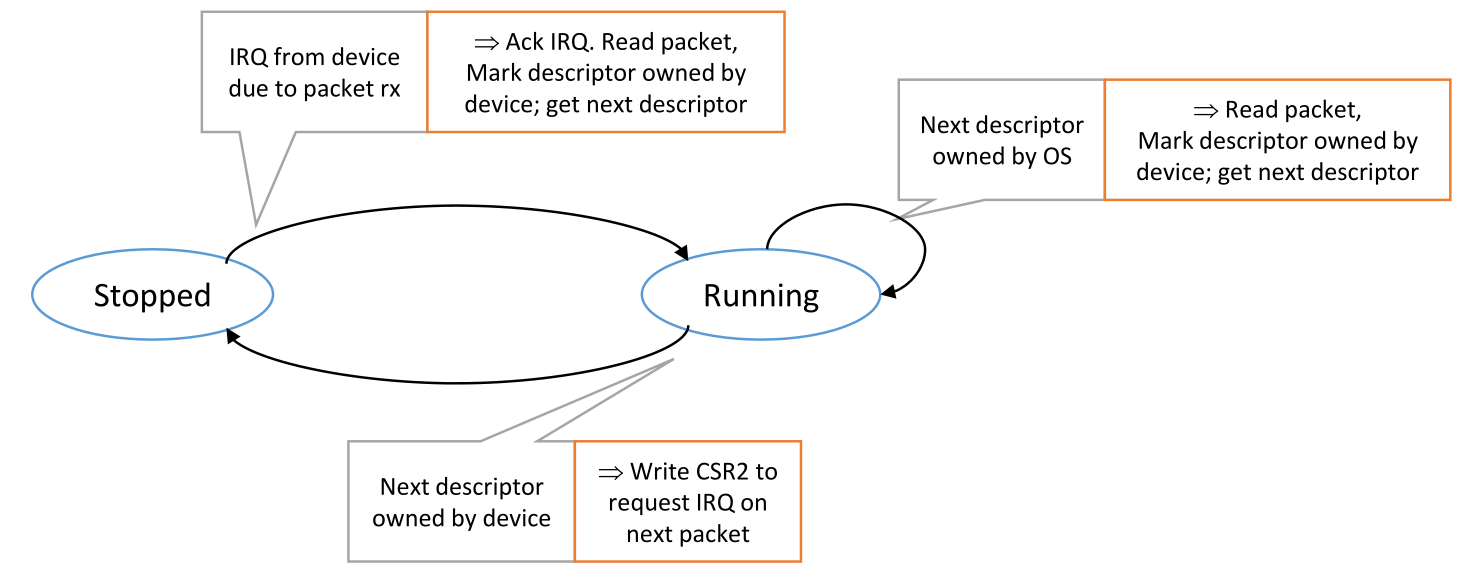
\includegraphics[width=0.8\textwidth]{25_StateMachineOsReceive.png}

\subsubsection{Discoverable Buses: PCI}
How does the OS know what devices are plugged in, how does it keep track of the addresses of each device (where are the registers of these devices)... There are many open question regarding the connection of devices.

We look at PCI as a particular solution to this problem.

PCI stands for \textit{Peripheral Component Interconnect}. It is a standard for connecting devices to a computer and also standards the physical connectors (the ones sitting on a motherboard). It also defines the bus protocol and how messages are interpreted by the CPU und devices. It is kind of the software-visible interface to IO hardware.

PCIe (PCI-Express) is the successor of PCI, but we still consider PCI in this course since the general principle is the same.

PCIe is a high speed serial connector ($O(1GB/s)$) while PCI is a parallel connector ($O(100MB/s)$).

\paragraph{PCI Solves}
PCI allow to discover devices and keep track of addresses. It also helps to map interrupts to exception vectors. It also provides a DMA. This allows devices to initiate DNA requests (this used to be initiated by the CPU).

\paragraph{Physical Connections}
PCI can be seen as a tree. 

The PCI root bridge (PCI root complex) connects the PCI to the main memory bus. Through other bridges, PCI is connected to other things like USB, SATA, NIC etc.

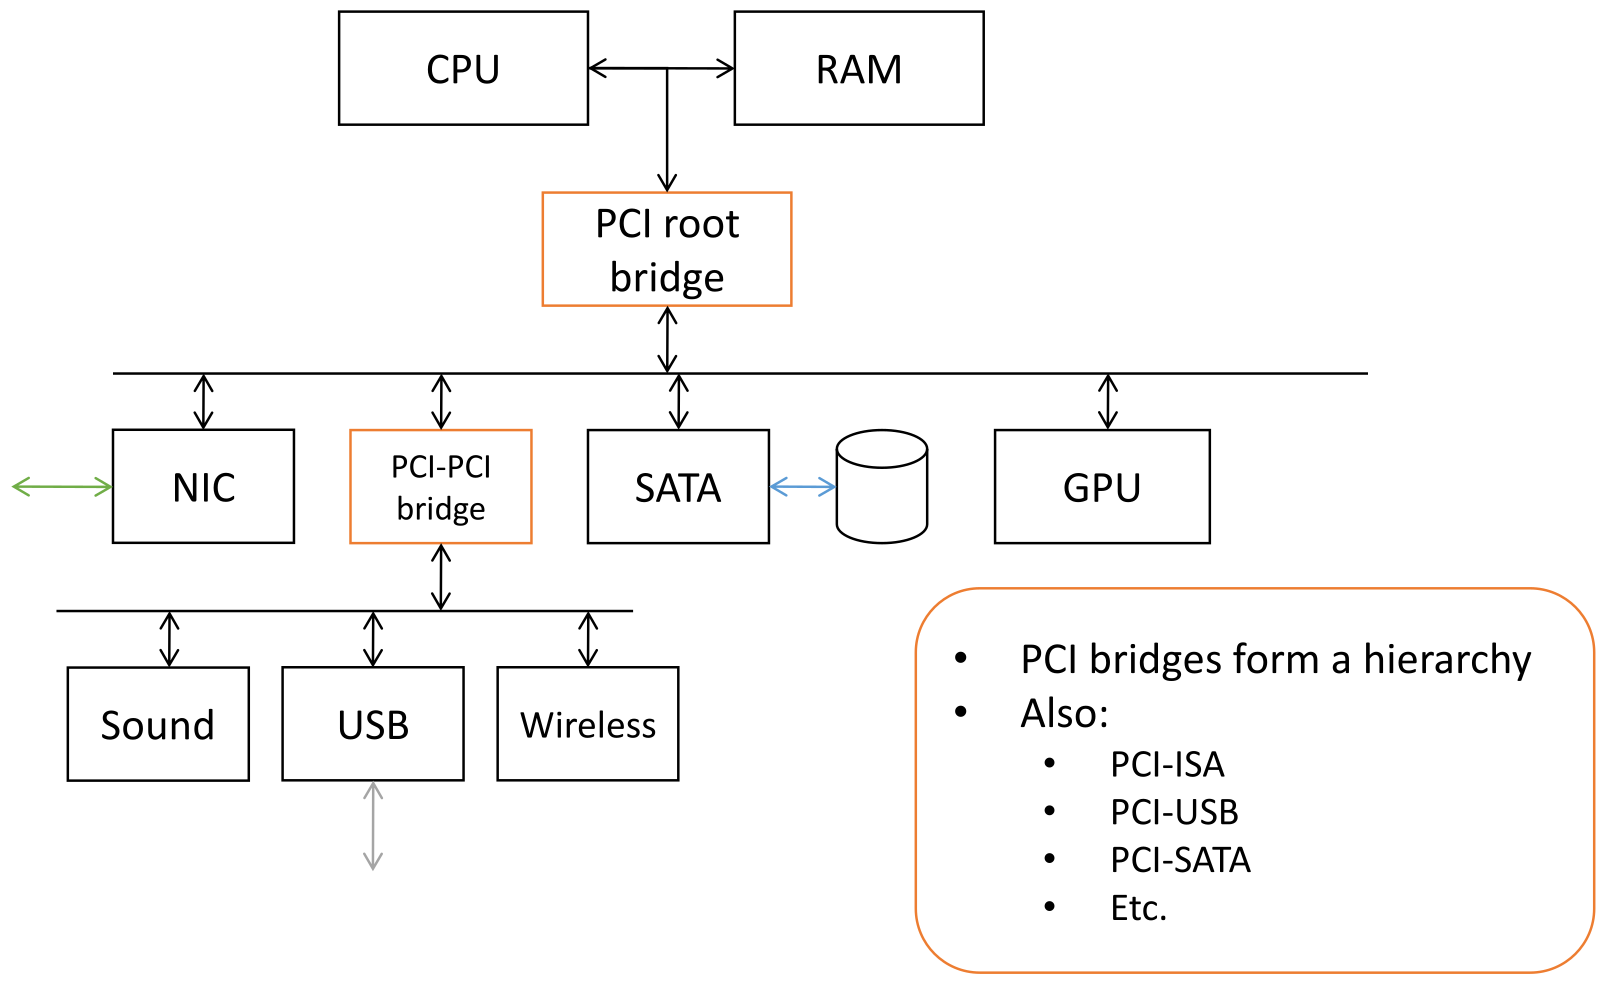
\includegraphics[width=0.8\textwidth]{25_PciTree.png}

\paragraph{Address Space}
The PCI address space is flat. This means that it is one big address space for all devices. Each device asks for a set of addresses in this range. Physical address space is usually $32$ or $64$-bits and the I/O address space is usually $16$-bit.

The PCI bridges remap addresses to the device. This is required since the PCI addresses may not be contiguous while the device required contiguous addresses

\paragraph{PCI Devices}
PCI devices are self describing. This means that they have all information required to identify them. This included vendor, model, version etc.

\paragraph{Finding All The Devices}
The first thing we do is finding the root bridge. In large systems there may be multiple such root bridges. Then we read the configuration of each device. While iterating the we add them to a list and record the size of the required address space. If we find a bridge, we do recursively discover it.

This results in a list of all devices and there address space requirements.

\paragraph{Allocating Addresses}
We find a suitable address range for each device following the requirements:
\begin{itemize}
    \item Required address space size of device must match
    \item All devices of a bridge must fit into the address space range of the bridge of that bus.
    \item The range is aligned as a power of $2$
\end{itemize}

Then we must program the address translation information. For each device we must save the base address of that device. This is stored in the \textit{base-address/range (BAR)} register.

\paragraph{PCI Interrupts}
There are four interrupt lines (INTA, INTB, INTC, INTD). When a PCI bus detects a interrupts, it forwards it to the root bridge which then interrupts the CPU. 

PCIe introduces \textit{message-signaled interrupts (MSIs)}. Instead of settings a physical pin of the CPU, we can set a certain memory mapped address. This will signal the right interrupt to the CPU. So interrupts are sent to specific addresses and depending on the address a different interrupt is sent. This reduces the need of pins on the CPU.
